\documentclass[11pt]{article}

\usepackage{times}
\usepackage{amsfonts}
\usepackage{amsmath}
\usepackage[psamsfonts]{amssymb}
\usepackage{latexsym}
\usepackage{color}
\usepackage{graphics}
\usepackage{enumerate}
\usepackage{amstext}
\usepackage{url}
\usepackage{epsfig}
\usepackage{bm}
\usepackage{hyperref}
\hypersetup{
    colorlinks=true,
    linkcolor=blue,
    filecolor=magenta,      
    urlcolor=blue,
}
\usepackage{mathtools}
 \usepackage{tikz}
\usetikzlibrary{shapes.geometric, arrows, positioning, shapes}
\usetikzlibrary{positioning}
\tikzstyle{startstop} = [rectangle, rounded corners, minimum width=3cm, minimum height=1cm,text centered, draw=black, fill=red!30]
\tikzstyle{io} = [trapezium,trapezium left angle=70,trapezium right angle=-70,minimum height=0.6cm, draw, fill=blue!20, text width=4.5em, text badly centered, node distance=3cm, inner sep=0pt]
\tikzstyle{process} = [rectangle, minimum width=3cm, minimum height=1cm, text centered, text width=3cm, draw=black, rounded corners, fill=orange!30]
\tikzstyle{decision} = [diamond, minimum width=3cm, minimum height=1cm, text centered, draw=black, fill=blue!20]
\tikzstyle{arrow} = [thick,->,>=stealth]
\tikzstyle{line} = [draw, -latex']
\tikzstyle{assignment} = [trapezium, trapezium left angle=80, trapezium right angle=100, minimum height=1cm, text centered, draw=black, fill=blue!30, text width=4.5cm]
\tikzstyle{block} = [rectangle, draw, fill=blue!20, text width=5em, text centered, rounded corners, minimum height=4em]
\tikzstyle{cloud} = [draw=orange, circle, thick,  minimum height=2em]

\def\Kset{\mathbb{K}}
\def\Nset{\mathbb{N}}
\def\Qset{\mathbb{Q}}
\def\Rset{\mathbb{R}}
\def\Sset{\mathbb{S}}
\def\Zset{\mathbb{Z}}
\def\squareforqed{\hbox{\rlap{$\sqcap$}$\sqcup$}}
\def\qed{\ifmmode\squareforqed\else{\unskip\nobreak\hfil
\penalty50\hskip1em\null\nobreak\hfil\squareforqed
\parfillskip=0pt\finalhyphendemerits=0\endgraf}\fi}

\DeclarePairedDelimiter{\nint}\lfloor\rceil
\DeclareMathOperator*{\E}{\rm E}
\DeclareMathOperator*{\argmax}{\rm argmax}
\DeclareMathOperator*{\argmin}{\rm argmin}
\DeclareMathOperator{\sgn}{sign}
\DeclareMathOperator{\supp}{supp}
\DeclareMathOperator{\last}{last}
\DeclareMathOperator{\sign}{\sgn}
\DeclareMathOperator{\diag}{diag}
\providecommand{\abs}[1]{\lvert#1\rvert}
\providecommand{\norm}[1]{\lVert#1\rVert}
\def\vcdim{\textnormal{VCdim}}

\DeclarePairedDelimiter\ceil{\lceil}{\rceil}
\DeclarePairedDelimiter\floor{\lfloor}{\rfloor}

\newcommand{\cX}{{\mathcal X}}
\newcommand{\cY}{{\mathcal Y}}
\newcommand{\cA}{{\mathcal A}}
\newcommand{\ignore}[1]{}
\newcommand{\bi}{\begin{itemize}}
\newcommand{\ei}{\end{itemize}}
\newcommand{\be}{\begin{enumerate}}
\newcommand{\ee}{\end{enumerate}}
\newcommand{\bd}{\begin{description}}
\newcommand{\ed}{\end{description}}
\newcommand{\h}{\widehat}
\newcommand{\e}{\epsilon}
\newcommand{\mat}[1]{{\mathbf #1}}
\newcommand{\R}{\mat{R}}
\newcommand{\0}{\mat{0}}
\newcommand{\M}{\mat{M}}
\newcommand{\D}{\mat{D}}
\renewcommand{\r}{\mat{r}}
\newcommand{\x}{\mat{x}}
\renewcommand{\u}{\mat{u}}
\renewcommand{\v}{\mat{v}}
\newcommand{\w}{\mat{w}}
\renewcommand{\H}{\text{0}}
\newcommand{\T}{\text{1}}
\newcommand{\set}[1]{\{#1\}}
\newcommand{\xxi}{{\boldsymbol \xi}}
\newcommand{\ssigma}{{\boldsymbol \sigma}}
\newcommand{\Alpha}{{\boldsymbol \alpha}}
\newcommand{\tts}{\tt \small}
\newcommand{\hint}{\emph{hint}}
\newcommand{\matr}[1]{\bm{#1}}     % ISO complying version
\newcommand{\vect}[1]{\bm{#1}}     % ISO complying version
\renewcommand{\labelitemi}{$\bullet$}
\renewcommand{\labelitemii}{$\cdot$}
\renewcommand{\labelitemiii}{$\diamond$}
\renewcommand{\labelitemiv}{$\ast$}

\newenvironment{solution}{\vspace{.25cm}\noindent{\it Solution:}}{}

\begin{document}

\noindent DS-GA 1008\\
Deep Learning, Spring 2019\\
Homework Assignment 3 \\
Yves Greatti - yg390\\
\href{https://www.overleaf.com/project/5c8521e162afe55c8eda31eb}{Read-Only Link to tex file}


\section*{1. Fundamentals}

\subsection*{1.1. Dropout}

\begin{itemize}
    \item[(a)]    The 2D dropout  technique is implemented by torch.nn.Dropout2d(p=0.5, inplace=False)
    \item[(b)]  
Deep neural networks, with non-linear "hidden" layers, will model almost perfectly complex relationships between the input and the correct output and there will be many different settings of the weight vectors. Each of these instance of trained neural network, will do worse on the test data than on the training data, and in essence they will overfit. With unlimited resources, the best way to "regularize" a network is to average the settings of all these weight vectors. Dropout is a cheap albeit efficient method of regularizing. Dropout provides an approximation to model combination  in evaluating a bagged ensemble of exponentially many neural networks.  It helps the network to not give too much importance to a particular feature. It helps to learn robust features which are more useful with many different random subsets. It also helps to reduce interdependence amongst the neurons, and limits the network ability to memorize very specific conditions during training.\\
Dropping out could apply to input and hidden units ,which mean they are temporarily removed from the network. In the simplest case, each unit is retained with a fixed probability $p$ independent of other units, $p$ is an hyperparameter which can be chosen using a validation set or is fixed. Typically, 0.5 for a hidden unit seems the optimal value for a wide range of networks and tasks and for the input units, the  value is closer to 1 like 0.8.\\
In practice, for each minibatch a random binary mask is applied to all the input and hidden units of a layer, the mask is generated independently for each dropout layer. If a unit in a layer, is retained with a probability $p$ during training, the outgoing outgoing weights of that unit are multiplied by $p$ at test time: the output at test time is same as expected output at training time.\\ PyTorch torch.nn.Dropout implementation to keep the inference as fast possible scales the units using the reciprocal of the keep probability $\frac{1}{1-p}$ during training which yields the same result. 2D dropout in PyTorch performs the same function as the previous one, however it drops the entire 2D feature map instead of individual unit. In early convolution layers adjacent pixels within each feature maps are strongly correlated, the regular dropout will not regularize the activations and, instead spatial dropout 2D helps in promoting independence between feature maps and should be preferred instead. Because dropout is a regularization technique, it reduces the capacity of the network, which leads to an increase of its size and the number of iterations (epochs) during training. However training time for each epoch is less. In very large datasets, regularization does not have a direct impact on the generalization error, in these cases, dropout could be less relevant. On very small training examples, dropout is less effective compared to \textbf{bayesian networks}. Dropout has inspired other approaches like \textbf{fast dropout}, or \textbf{drop out boosting} but none of them have outperformed its performances.
 

\end{itemize}
\subsection*{1.2. Batch Norm}

\begin{itemize}
    \item[(a)]   What does mini-batch refer to in the context of deep learning?\\
    Mini-batch in the context of deep learning is related to the batch size of the data used by the gradient descent algorithm that splits the training
    data into small batches that are used to compute model error and update its parameters. It seeks to combine the effects of batch gradient descent and stochastic gradient descent.
    In batch gradient descent, the gradient is computed over the entire dataset. In stochastic gradient descent, the gradient is computed on a single instance of the dataset. On expectation, the gradient on a random sample will point to the same direction of the full dataset samples. SGD is more efficient and its stochastic property  can allow the model to avoid local minima.  SGD actually, helps generalization by finding "flat" minima on the training set, which are more likely to also be minima on the test set (see \href{https://cbmm.mit.edu/sites/default/files/publications/CBMM-Memo-067.pdf}{Theory of Deep Learning III: Generalization Properties of SGD}). Minibatch will have a size ranging from 2 to 32 (see \href{https://arxiv.org/abs/1804.07612}{Revisiting Small Batch Training for Deep Neural Networks}). Minibatch, compared to SGD, can still be parallelized.
    \item[(b)]
    Batch normalization reduces the \textit{"Internal Covariate Shift"} which is defined in \href{https://arxiv.org/abs/1502.03167}{Batch Normalization: Accelerating Deep Network Training by Reducing Internal Covariate Shift}, as the change in the distribution of network activations due to the change in network parameters during training: inputs to each layer are affected by the parameters of all preceding layers. Before batch normalization, saturated regime of non-linear activation resulting in vanishing gradient, were usually addressed by using Relu, small learning rates or careful initialization of the weights. Batch normalization helps to avoid these issues by subtracting the mean and dividing by the batch standard distribution, normalizing the scalar feature to have a Gaussian distribution $\mathcal{N}(0,1)$.  In implementation, this technique usually amounts to insert the BatchNorm layer immediately after the fully connected layer or convolutional layer, and before non-linearities. Batch normalization, by preventing the model from getting stuck in the saturated regime of nonlinearities, enables higher learning rates and allows to achieve faster training. By whitening the inputs of  each layer, BatchNorm regularizes the model removing or reducing the need for dropout. After the shift and scaling, two learnable parameters, $\gamma$ and $\beta$, are used to avoid the network to undo the normalization and recover the original activations  of the network. The output of a BatchNorm layer is given by:
    	\[
    		y =\frac{x-E[x]} {\sqrt{Var[x]+\epsilon}} * \gamma + \beta
    	\]
	In PyTorch,  by default, the elements of $\gamma$ are sampled from a uniform distribution $\mathcal{U}(0,1)$ and the elements of $\beta$ are set to 0. The mean and standard deviation are computed over the mini-batches and each layer can keep running estimates using a momentum. The running averages for mean and variance are updated using an exponential decay based on the momentum parameter:
	\begin{itemize}
    		\item running\_mean = momentum * running\_mean + (1 - momentum) * sample\_mean (sample\_mean is the new observed mean)
    		\item running\_var = momentum * running\_var + (1 - momentum) * sample\_var (sample\_var is the new observed variance)
    	\end{itemize}   
	momentum=0 means that old information is discarded completely at every time step, while momentum=1 means that new information is never incorporated. For fully connected activation layers, BN is applied separately to each dimension (H, W) with a pair of learned parameters $\gamma$ and $\beta$ per dimension. For convolutional layers, BN is applied so that different elements of the same feature map, at different spatial locations, are normalized across the mini-batch. The parameters $\gamma$ and $\beta$ are learned per feature map. BN is a differentiable transformation and using the chain rules the gradient of loss can be explicitly formalized and it can be shown that backpropagation for BN is unaffected by the scale of its parameters and BN will stabilize the parameter growth. 
 \end{itemize}   
 
 \section*{2. Language Modeling}
 
 This exercise explores the code from the \href{https://github.com/pytorch/examples/tree/master/word_language_model}{word\_language\_model} example in PyTorch.
 \begin{itemize}
   \item[(a)]   
   Go through the code and draw a block diagram / flow chart (see this \href{https://www.sharelatex.com/blog/2013/08/29/tikz-series-pt3.html} {tutorial}) which highlights the main interacting components, illustrates their functionality, and provides an estimate of their computational time percentage (rough profiling).
   
   \subsection*{Main Component}
   We start to describe the  major functions used in the main component flow chart.
   \begin{itemize}
   	\item \textbf{Read corpus data} creates three dictionaries: train, validation and test from three separate related files (train.txt, valid.txt, test.txt). Each line of a text file is split in words, and each word
	is added to a dictionary. A dictionary is made of two maps: (1) word to index: word2idx and (2) index to word: idx2word.
	\item \textbf{batchify()} given a tensor of size M, the function creates N batches of size batch\_size ($N=\nint{M/\text{batch\_size}}$), throwing away the data in excess of N. 
	Starting from sequential data, batchify arranges the dataset into columns. For instance, with the alphabet as the sequence and batch size of 4, we will get
	\[
			\begin{bmatrix}
   				\text{a} &  \text{g} & \text{m} & \text{s}  \\
   				\text{b}  &  \text{h} & \text{n} & \text{t} \\
   				\text{c}  &  \text{i} & \text{o} & \text{u} \\
   				\text{d}  &  \text{j} & \text{p} & \text{v} \\
   				\text{e}  &  \text{k} & \text{q} & \text{w} \\
   				\text{f}  &  \text{l} & \text{r} & \text{c} \\
			\end{bmatrix}
	\]	
	These columns are treated independently without trying to learn the dependency between characters like for e.g. between f and g but allows  more efficient batch processing.

   \end{itemize}
   \vspace{2mm}
   
      \begin{center}
        \begin{tikzpicture}[node distance = 2cm]
       		\node (start) [startstop] {Start};
		\node (in1) [io, below of=start, node distance = 2cm] {Parse program arguments in \textit{args}};
		\node(b1)   [block, below of=in1, node distance = 2cm] {Set random seed\\Set device};
       		\node(b2)  [block, below of=b1, text width=10em, node distance = 2cm] {Set batch size for validation and test datasets to 10};
		\node (in2) [io, below of=b2, text width=4cm, node distance = 2cm] {Read corpus data};
      		\node(b3)  [block, below of=in2,  text width=10cm, node distance = 2cm]  {train\_data = \textit{batchify}(corpus.train, batch\_size) \\
																 val\_data = \textit{batchify}(corpus.valid, eval\_batch\_size) \\
																 test\_data= \textit{batchify}(corpus.test, eval\_batch\_size) };      
      		\node(b4)  [block, below of=b3,  text centered, text width=10cm]  {ntokens = length of vocabulary (length of \textit{dictionary})\\
																criterion = crossEntropyLoss};
      		\node(b5)  [block, below of=b4,  text width=10cm]  {model = model.RNNModel(args.model, ntokens, args.emsize, args.nhid, args.nlayers, args.dropout, args.tied)};
		\node(c1) [cloud, below of=b5, node distance = 2cm]  {1};
		 
		 % Draw edges
		 \path [line] (start) -- (in1);
		 \path [line] (in1) -- (b1);
		 \path [line] (b1) -- (b2);
		 \path [line] (b2) -- (in2);
		 \path [line] (in2) -- (b3);
		 \path [line] (b3) -- (b4);
		 \path [line] (b4) -- (b5);
		 \path [line] (b5) -- (c1);
        
        \end{tikzpicture}
    \end{center}

      \begin{center}
        \begin{tikzpicture}[node distance = 2cm, auto]
	         \node(c1)  [cloud]  {1};
	         \node(b1)  [block, below of=c1, text width=3cm] {epoch = 1\\ lr = args.lr};
	         \node(d1)  [decision, below of=b1, text width=3cm, node distance=3cm]{epoch $\le$ args.epoch};
		\node [right of=d1, xshift=0.5cm, yshift=0.2cm]  {no};
		
		% Main flow
	         \node(p1)  [process, below of=d1, node distance=3cm] {\textbf{train()}};
	         \node(p2)  [process, below of=p1, text width=5cm, node distance = 2cm] { val\_loss = \textbf{evaluate}(val\_data)};
	         \node(d2)  [decision, below of=p2,  text width=3cm, node distance=3cm]{val\_loss $<$ best\_val\_loss};
	         \node(b2)  [block, left of=d2, text width=3cm, xshift=-3cm] {Save model};
	         \node(b3)  [block, below of=b2, text width=4cm] {best\_val\_loss = val\_loss};
	         \node(b4)  [block, right of=d2, text width=3cm, xshift=3cm] {lr = lr $/$ 4};
		 \node(b5)  [block, below of=d2, text width=4cm, node distance=4cm] {epoch = epoch + 1};

	         \node(p3)  [process, right of=p1, xshift=4cm]{Load best model};
	         \node(p4)  [process, right of=p2, xshift=4cm] {test\_loss = \textbf{evaluate}(test\_data)};
	         \node (stop) [startstop, below of=p4, node distance=1.4cm] {Stop};


		 % Draw edges
		 \path [line] (c1) -- (b1);
		 \path [line] (b1) -- (d1);
		 \path [line] (d1) -- node  {yes} (p1);
		 \path [line] (p1) -- (p2);
		 \path [line] (p2) -- (d2);
		 \path [line] (d2) -- node [near start]  {yes} (b2);
		 \path [line] (d2) -- node {no} (b4);
		 \path [line] (b2) -- (b3);
		 \path [line] (b3) |- (b5);
		 \path [line] (b4) |- (b5);
	         \path [line] (b5.south) -- ++(0, -1.2) -- ++(-7.5, 0) -- ++(0, 5) |- (d1.west);
		 
		 \path[line]  (d1) -| (p3);
		 \path[line]  (p3) -- (p4);
		 \path [line] (p4) -- (stop);
	         
        \end{tikzpicture}
    \end{center}

   \subsection*{Main.train() Component}
      	The main functions of the train function are:
	\begin{itemize}

	\item \textbf{model.init\_hidden()}  assigns the initial hidden state of the recurrent neural network to a device (CPU or GPU)
	if the model and its parameters are on cpu, the same gpu if the model has been transferred with model.cuda()
	(see \href{https://github.com/pytorch/pytorch/blob/master/docs/source/notes/cuda.rst}{device-agnostic code}).
	\item \textbf{get\_batch()} will  generate chunks of length args.bptt, which corresponds to the length of the sequence being passed to the RNN model (sequence length) 
	Wit a bptt of 2 and reusing the previous example of the output of the batchify function, the function generates: 
	\[ \text{data}=\left(  \begin{array}{cccc}
			\text{a} &  \text{g} & \text{m} & \text{s}  \\
			\text{b}  &  \text{h} & \text{n} & \text{t}
		   \end{array} \right)
	 \text{target}=\left(\begin{array}{cccc}
			\text{c}  &  \text{i} & \text{o} & \text{u} \\
			\text{d}  &  \text{j} & \text{p} & \text{v}
		\end{array} \right)
	\]
	\item \textbf{repackage\_hidden(hidden)}  At each loop in the train() function, the RNN model is trained on a sequence of new characters produced by the  get\_batch() function and the gradients are backpropagated (BPTT) through the RNNs computational graph. From one iteration of the loop to the next iteration, if the hidden states from the previous iteration were still have a reference to the graph, the gradients will be backpropagated through them. This is not the intended behavior as we want the RNN's gradients to be propagated independently for each batch of words (sequence). To get rid of the references of the hidden states, repackage\_hidden(hidden) function wraps these hidden states into brand new tensors that have no history. This allows the previous graph to go out of scope and free up the memory for the next iteration.
	\item \textbf{Clipping the gradients:} is performed using  torch.nn.utils.clip\_grad\_norm. During the backpropagation, gradients are not clipped until the backward pass is completed and before the model parameters are updated.
	\end{itemize}
		   
         \begin{center}
         \begin{tikzpicture}[node distance = 2cm, auto]
        
               	\node (start) [startstop] {Start};
		\node(b1)  [block, below of=start] {model.train()};
		\node(b2)  [block, below of=b1, text width=5cm] {total\_loss = batch = i = 0\\hidden = model.init\_hidden()};
		\node(d1) [decision, below of=b2, yshift=-1.5cm]{i $<$ train\_data.size(0) - 1};
		\node [below of=d1, xshift=1.3cm]  {yes};
		\node(b3)  [block, below of=d1,  text width=5cm, yshift=-1.5cm] {data, targets = get\_batch(train\_data, i)};
		\node(b4)  [block, below of=b3,  text width=5cm] {hidden = repackage\_hidden(hidden)};
		\node(b5)  [block, below of=b4,  text width=5cm] {Set gradient of all model parameters to zero:\\ model.zero\_grad()};
		\node(p1) [process, below of=b5, text width=5cm, yshift=-0.4cm] {Pass data and hidden to RNN model:\\ output, hidden = model(data, hidden)};
		\node(c1)  [cloud, below of=p1, yshift=-0.1cm] {1};
	        \node (stop) [startstop, right of=d1, xshift=4cm] {Stop};
		\node(c2)  [cloud, right of=d1, xshift=-5cm] {2};

		 % Draw edges
		 \path [line] (start) -- (b1);
		 \path [line] (b1) -- (b2);
		 \path [line] (b2) -- (d1);
		 \path [line] (d1) -- (b3);
		 \path [line] (b3) -- (b4);
		 \path [line] (b4) -- (b5);
		 \path [line] (b5) -- (p1);
		 \path [line] (p1) -- (c1);
		 \path [line] (d1) -- node {no} (stop);
		 \path [line] (c2) -- (d1);

         \end{tikzpicture}
    \end{center}
    
    \begin{center}
         \begin{tikzpicture}[node distance = 2cm, auto]
		\node(c1) [cloud, below of=p1]  {1};
		\node(p1)  [process, below of=c1,  text width=5cm]{Compute the cross entropy loss between model's output and targets};
		\node(p2)  [process, below of=p1,  text width=5cm] {Backpropagate loss:\\loss.backward()};
		\node(p3) [process, below of=p2,  text width=5cm] {Clip gradients to avoid exploding gradients};
		\node(p4) [process, below of=p3,  text width=5cm] {Use the gradients to update the model parameters};
		\node(b1)  [block, below of=p4,  text width=5cm]{total\_loss =  total\_loss + loss};
		\node(d1) [decision, below of=b1, text width=4cm, yshift=-2cm]{batch modulo args.log\_interval};
		\node(b2)  [block, below of=d1, text width=4cm, yshift=-2cm]{total\_loss =  0};
		\node(b3)  [block, right of=b2, xshift=4cm, text width=5cm] {i = i + args.bptt};
		\node(c2)  [cloud, below of=b3] {2};

		 % Draw edges
		\path [line] (c1) -- (p1);
		\path [line] (p1) -- (p2);
		\path [line] (p2) -- (p3);
		\path [line] (p3) -- (p4);
		\path [line] (p4) -- (b1);
		\path [line] (b1) -- (d1);
		\path[line] (d1) -- node {yes} (b2);
		\path [line] (d1) -| node {no} (b3);
		\path [line] (b2) -- (b3);
		\path [line] (b3) -- (c2);
		
         \end{tikzpicture}
    \end{center}

    \subsection*{Main.evaluate() Component}
      	There are not important functions in the evaluate() function which have not already been covered. The major differences with the train function  are:
	\begin{enumerate}
	\item No gradients are calculated, no backprogation is performed, no gradient clipping, no update of the model parameters with the gradients. Although the repackage\_hidden is invoked, it should not be necessary to do so.
	\item The function accepts the parameter data source so it can be invoked for the validation and test datasets.	
	\item At each iteration the loss is multiplied by the sequence length and added to the total loss. At exit, the evaluate function returns the total\_loss divided by the total size of the data source
	returning in effect the updated total loss.
	\end{enumerate}
	
    \begin{center}
         \begin{tikzpicture}[node distance = 2cm, auto]
        
               	\node (start) [startstop] {Start};
		\node (in1) [io, below of=start,  text width=3.5cm, node distance = 1.5cm] {Input data\_source};
		\node(p1) [process, below of=in1,  text width=5cm] {Set the model in evaluation mode:\\ disable dropout};
		\node(b1)  [block, below of=p1, text width=5cm] {total\_loss = i = 0\\hidden = model.init\_hidden()};
		\node(p2) [process, below of=b1,  text width=5cm, yshift=-0.5mm] {Disable gradient computation};
		\node(d1) [decision, below of=p2, yshift=-1.5cm]{i $<$ data\_source.size(0) - 1};
		\node(c2)  [cloud, right of=d1, xshift=-6cm] {2};
		\node [below of=d1, xshift=1.3cm]  {yes};
		\node(b2)  [block, below of=d1,  text width=5cm, yshift=-1.5cm] {data, targets = get\_batch(data\_source, i)};
		\node(b3)  [block, right of=b2, xshift=4cm, text width=5cm] {total\_loss = total\_loss / len(data\_source)};
		\node(c1)  [cloud, below of=b2, yshift=-0.1cm] {1};
	        \node (stop) [startstop, below of=b3, yshift=-1cm] {Stop};

		 % Draw edges
		\path [line] (start) -- (in1);
		\path [line] (in1) -- (p1);
		\path [line] (p1) -- (b1);
		\path [line] (b1) -- (p2);
		\path [line] (p2) -- (d1);
		\path [line] (d1) -- (b2);
		\path [line] (b2) -- (c1);
		\path [line] (d1) -| node {no} (b3);
		\path [line] (b3) -- (stop);
	         \path [line] (c2) -- (d1);

         \end{tikzpicture}
    \end{center}
    
    \begin{center}
         \begin{tikzpicture}[node distance = 2cm, auto]
        		\node(c1) [cloud, below of=p1]  {1};
		\node(p1)  [process, below of=c1,  text width=5cm]{Compute the cross entropy loss between model's output and targets};
		\node(b1)  [block, below of=p1,  text width=7cm]{total\_loss =  total\_loss + len(data) * loss};
		\node(b2)  [block, below of=b1, text width=5cm] {i = i + args.bptt};
		\node(c2)  [cloud, below of=b2] {2};
		
		 % Draw edges
		\path [line] (c1) -- (p1);
		\path [line] (p1) -- (b1);
		\path [line] (b1) -- (b2);
		\path [line] (b2) -- (c2);
		
         \end{tikzpicture}
    \end{center}
   
   \subsection*{Profiling}
   
   \subsubsection*{batchify}
   Most of the time as indicated in column \%Time is spent in the reshaping of the data (Fig. ~\ref{fig:batchify}).
   \begin{figure}[h!]
  		 \centering
 	 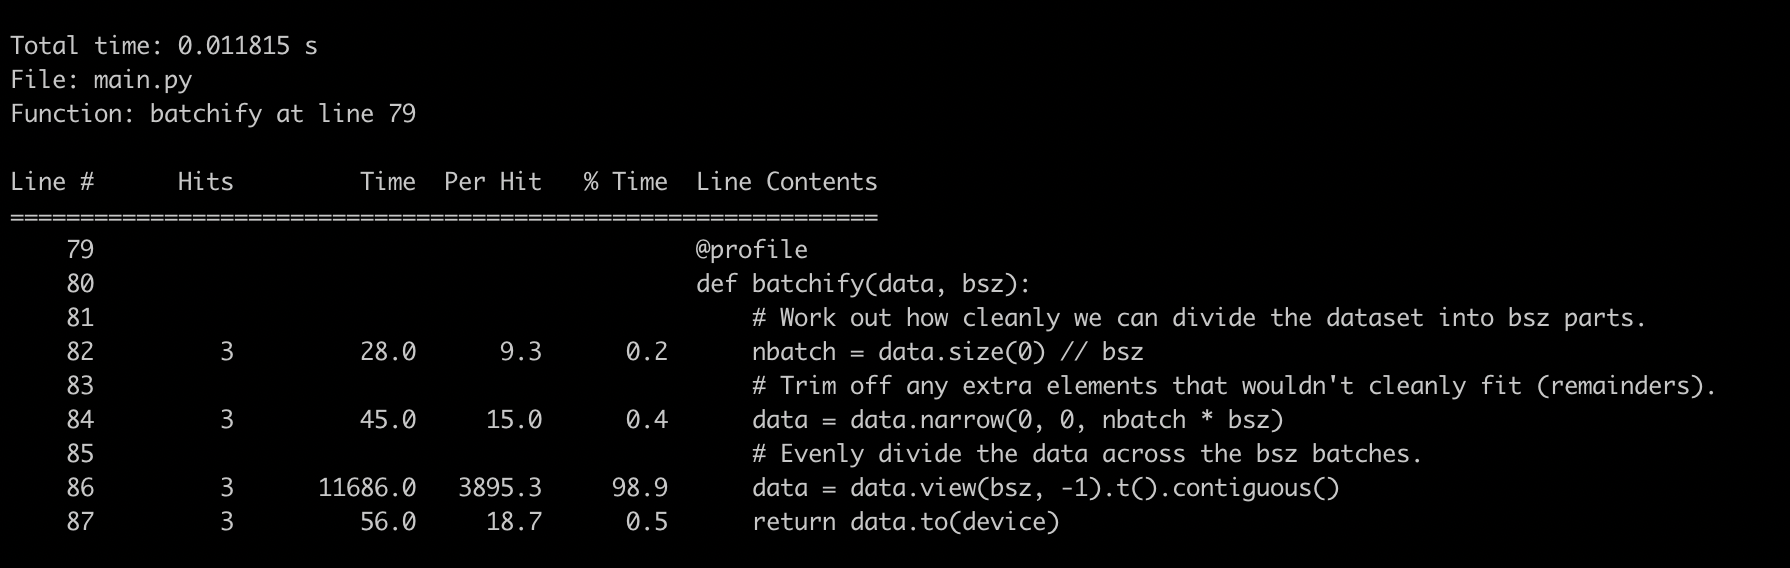
\includegraphics[width=\linewidth]{batchify.png}
 	 \caption{batchify.}
 	 \label{fig:batchify}
   \end{figure}

   \subsubsection*{repackage\_hidden}
   This is a recursive function, if the computational time percentages are not affected by the recursion: the time is equally spent across the function  (Fig. ~\ref{fig:repackagehidden}).
    \begin{figure}[h!]
         \centering
 	 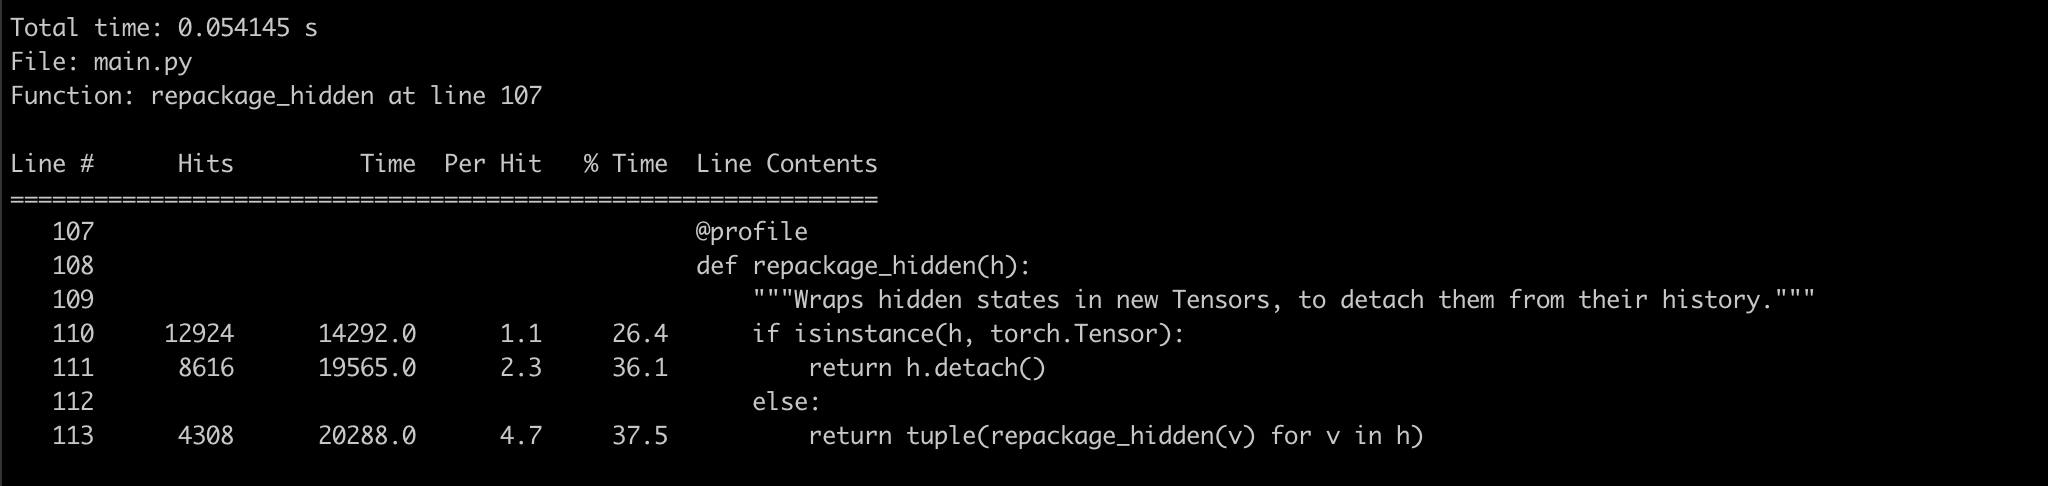
\includegraphics[width=\linewidth]{repackageHidden.png}
 	 \caption{repackage\_hidden.}
 	 \label{fig:repackagehidden}
   \end{figure}
   
   \subsubsection*{get\_batch}
   Another computational time uniformly distributed cross the function (Fig. ~\ref{fig:getbatch}).
   \begin{figure}[h!]
  	\centering
 	 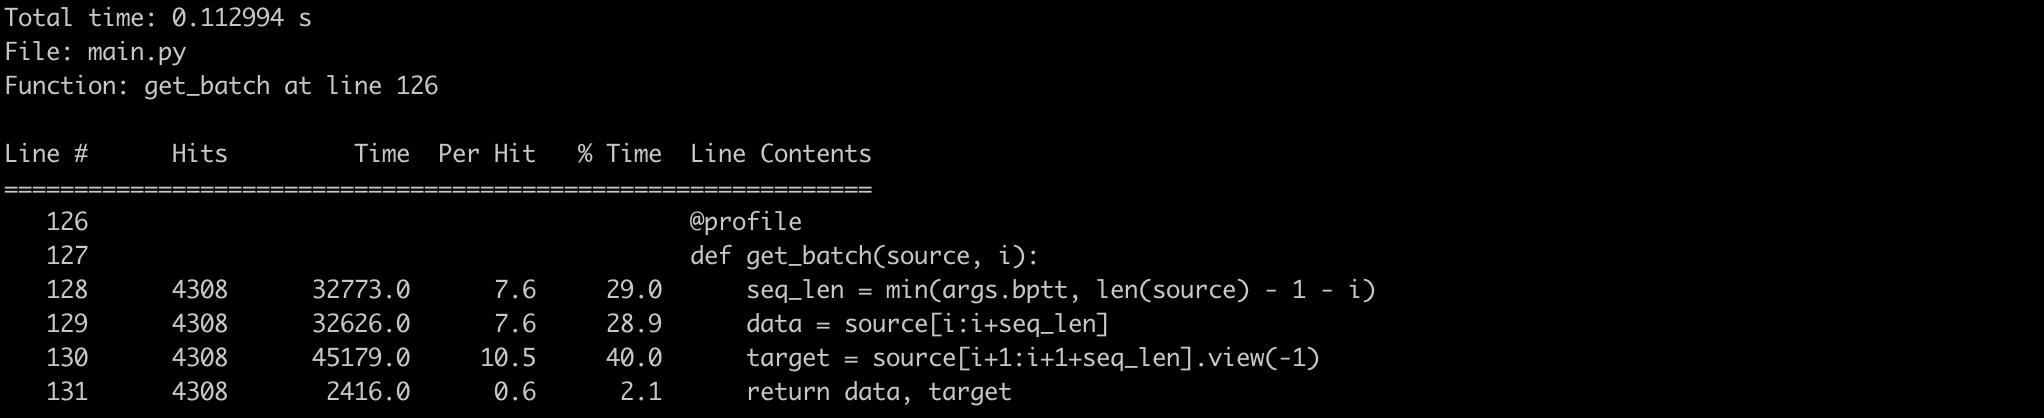
\includegraphics[width=\linewidth]{getBatch.png}
 	 \caption{get\_batch.}
 	 \label{fig:getbatch}
   \end{figure}

   \subsubsection*{train}
   The time is split between the forward pass executed by the model and the back-propagation triggered at line 165: loss.backward()  (Fig. ~\ref{fig:train}).
   \begin{figure}[h]
  	\centering
 	 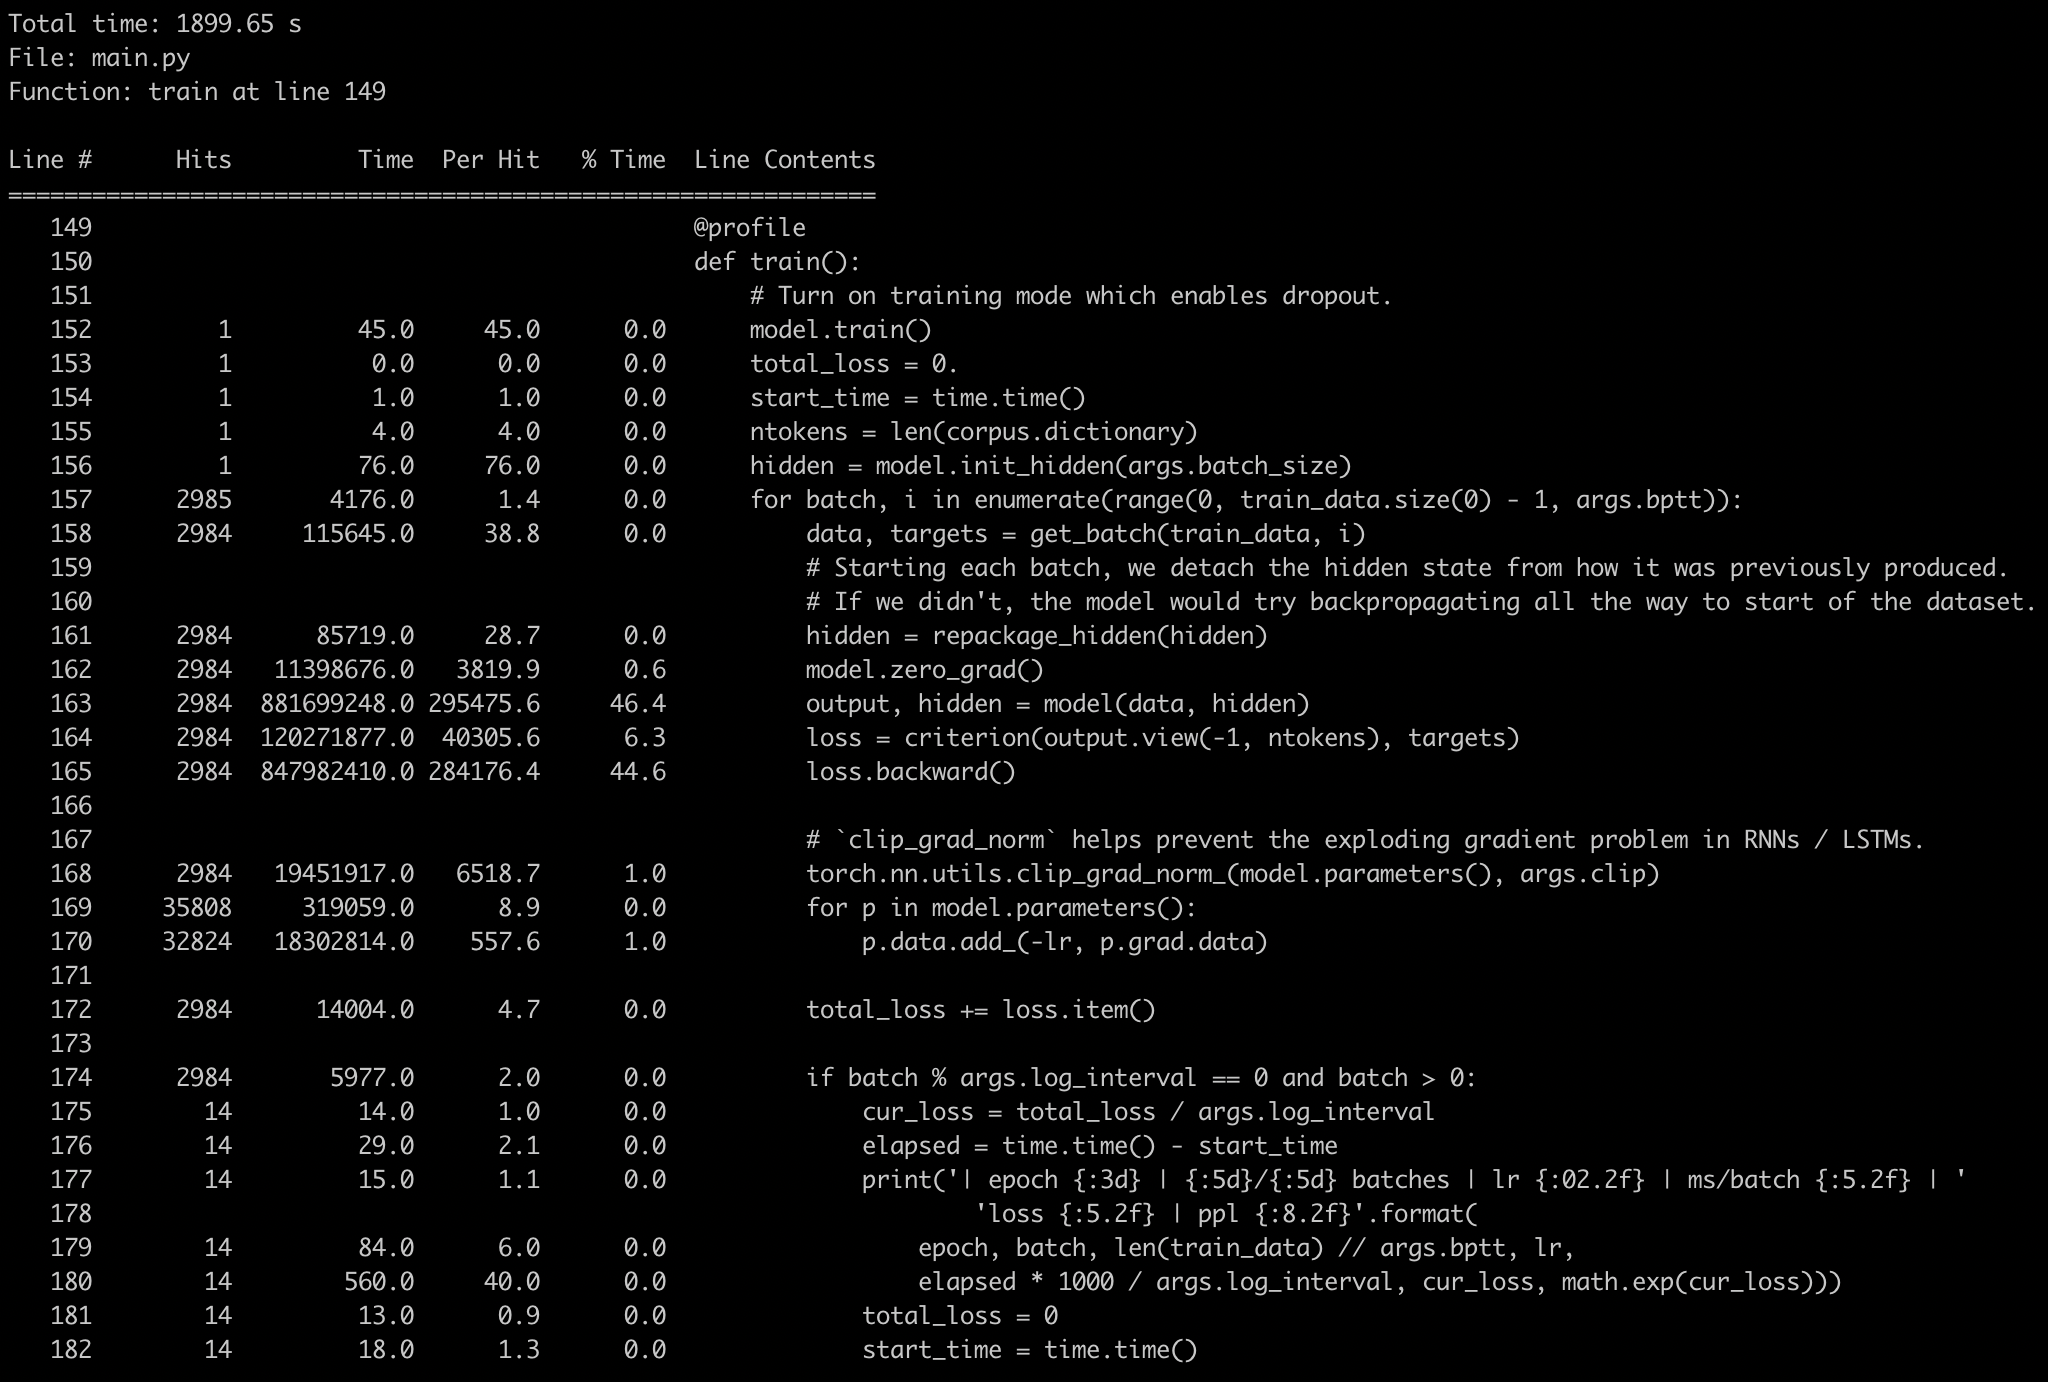
\includegraphics[width=\linewidth]{train.png}
 	 \caption{train.}
 	 \label{fig:train}
   \end{figure}


   \subsubsection*{evaluate}
   60\% of the time is spent inside the model processing the data and 30\% is taken by the computation of the loss (Fig. ~\ref{fig:evaluate}).
   \begin{figure}[h!]
  	\centering
 	 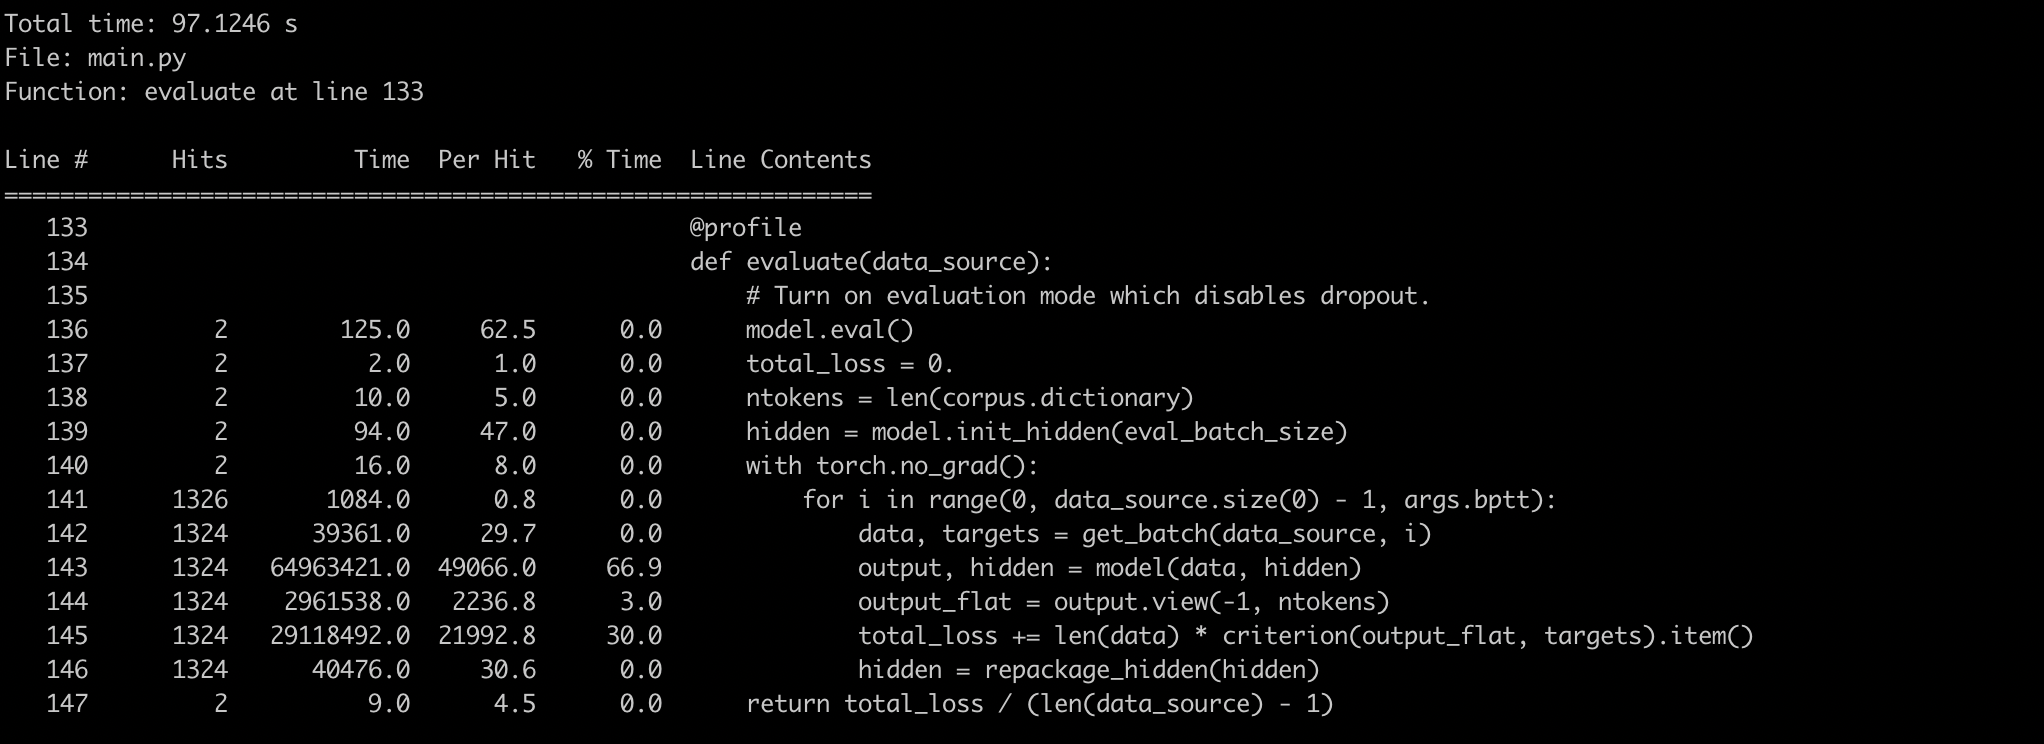
\includegraphics[width=\linewidth]{evaluate.png}
 	 \caption{evaluate.}
 	 \label{fig:evaluate}
   \end{figure}

  \subsubsection*{main flow}
   Most of the time, as you will expect, is spent within the train() function and  about 3\% (2.3\% and 2.6\%)  are consumed by the evaluation on the validation and test datasets (Fig. ~\ref{fig:main}).
   \begin{figure}[h!]
  	\centering
 	 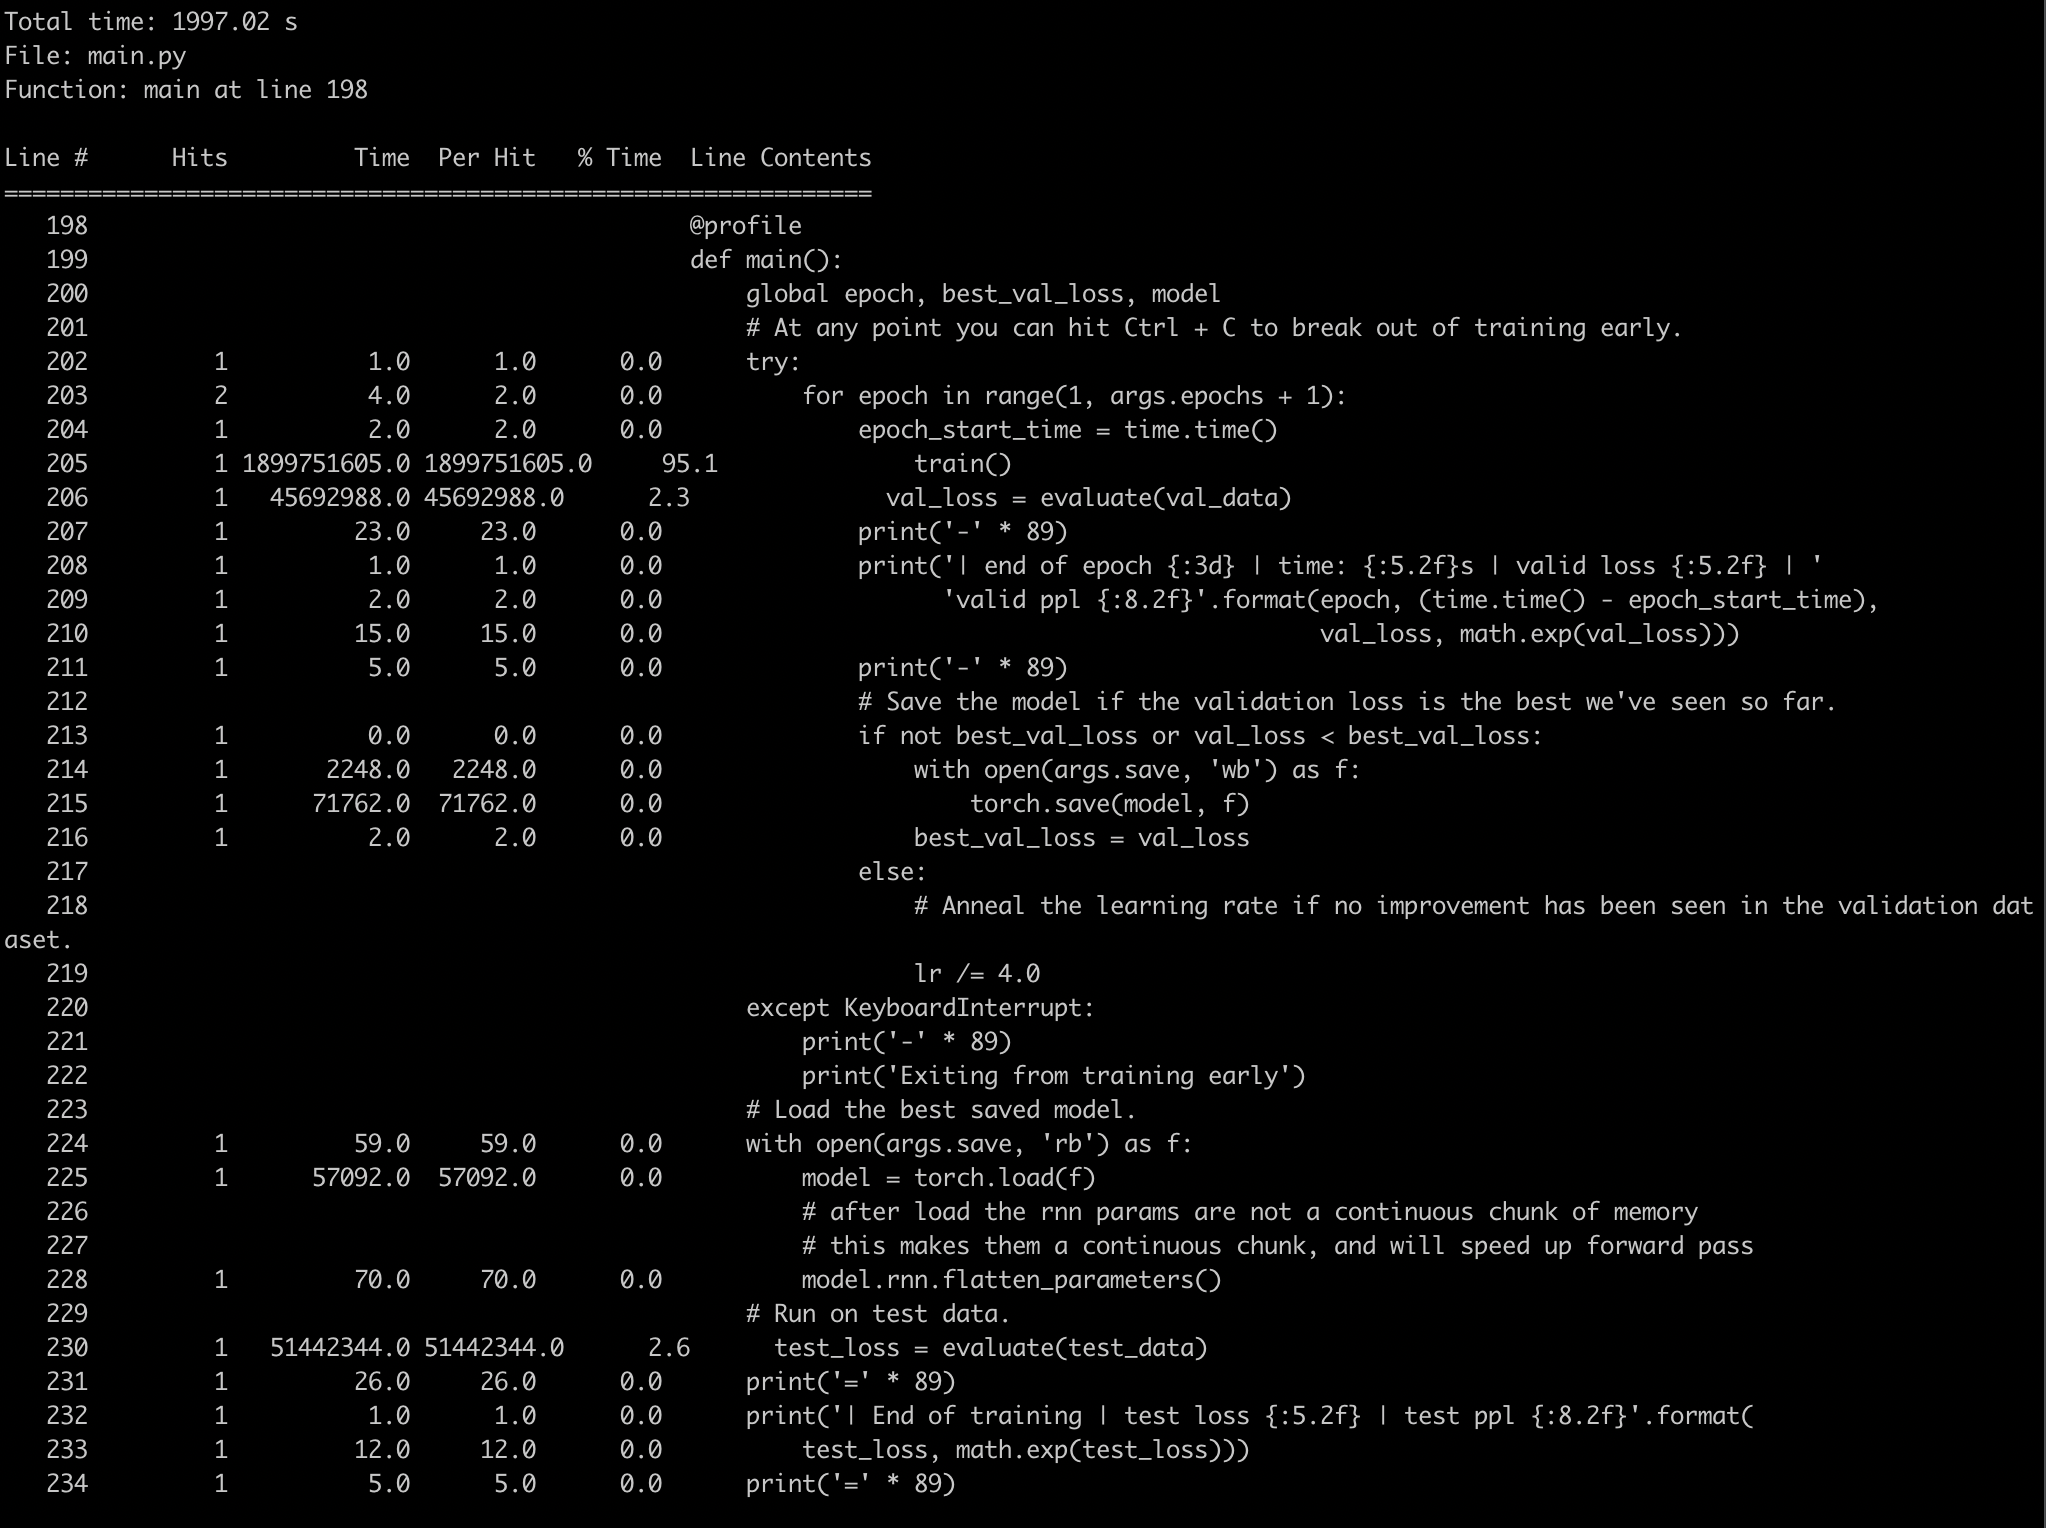
\includegraphics[width=\linewidth]{main.png}
 	 \caption{main.}
 	 \label{fig:main}
   \end{figure}

           
   \item[(b)]
   Find and explain where and how the back-propagation through time (BPTT) takes place (you may need to delve into PyTorch source code). 
   The backpropagation through time starts in the train function at the line: loss.backward(). The generalized back-propagation algorithm is applied to the unrolled computational graph $\vect{h}^(t) = f(\vect{h}^{t-1}, \vect{x}^t; \theta)$ where $\vect{h}^t$ represents the hidden state a time t and $\vect{x}^t$ the input $\vect{x}$ a time t and $\theta$ the model parameters.
   The RNNModel architecture is:
   \[
  	 \begin{tabular}{| c | c | c |}
  	  \hline
	  \text{Layer} & \text{Output Shape}  \\
	  \hline
	  \text{Linear} & \text{(args.nlayers, ntokens)}  \\
	  \hline
	  \text{Recurrent Network} & \text{(args.emsize, args.nlayers)}  \\
	  \hline
	  \text{Dropout} & \text{(ntokens, args.emsize)} \\
	  \hline
	  \text{Embedding} & \text{(ntokens, args.emsize)}  \\
	  \hline
	\end{tabular}
\] 
Recurrent Network is either LSTM, RNN\_TANH, RNN\_RELU or GRU. The back-propagation will trickle down starting from the loss, to the linear layer, through the recurrent network unrolled computational graph up to and including the embedding layer. BPTT refers to the back-propagation specific to the recurrent network seen as unrolled computational graph. It stops at line 158 with the line: hidden = repackage\_hidden(hidden) where the hidden states of the model are detached from the computational graph.
	
    \item[(c)]      
    Describe why we need the repackage\_hidden(h) function, and how it works.
 At each loop in the train() function, the RNN model is trained on a sequence of new characters produced by the  get\_batch() function and the gradients are backpropagated (BPTT) through the RNNs computational graph. From one iteration of the loop to the next iteration, if the hidden states from the previous iteration were still have a reference to the graph, the gradients will be backpropagated through them. This is not the intended behavior as we want the RNN's gradients to be propagated independently for each batch of words (sequence). To get rid of the references of the hidden states, repackage\_hidden(hidden) function  wraps these hidden states into, \textit{fresh}, new tensors that have no history. This allows the previous graph to go out of scope and free up the memory for the next iteration.
    
     \item[(d)] 
    Why is there a --tied (tie the word embedding and softmax weights) option?
    The model can be separated into two components:
    \begin{itemize}
     \item The encoder which takes a one hot vector of an input word, multiplies it by the a matrix to give a word embedding. 
     \item The decoder which multiplies the word embedding by another matrix resulting to an output embedding vector. This vector is then passed through a cross entropy loss, normalizing its values into a probability distribution.
    \end{itemize}
    Input embedding and output embedding have few common properties. The first property, they share is that they are both of the same size (args.emsize). The second property is that they will show similar behavior.
    The input embedding words with similar meanings, will be represented by similar vectors (in term of cosine similarity). Given the representation from the RNN, the decoder would like to assign similar probabilities to similar words.
    Therefore similar words are represented by similar vectors in the output embedding. Experiments have also shown that the word representations in the output embedding are of much higher quality than the ones in the input
    embedding. In a weight tied model, a single high quality embedding matrix is used in two places in the model. In addition weight tying reduces the number of parameters (increases training speed), and has a regularization effect
    as the model has less capacity to overfit.       
     \item[(e)] 
     Compare LSTM and GRU performance (validation perplexity and training time) for different values of the following parameters: number of epochs, number of layers, hidden units size, input embedding dimensionality, BPTT temporal interval, and non- linearities (pick just 3 of these parameters and experiment with 2-3 different values for each).
     \item[(f)] Why do we compute performance on a test set as well? What is this number good for?
 \end{itemize}   
 
\end{document}
